\documentclass[a4paper]{report}

\usepackage{graphicx}
\usepackage[english]{babel}
\usepackage[utf8]{inputenc}
\usepackage[T1]{fontenc}
\usepackage{ragged2e}
\usepackage{hyphenat}
\usepackage{lmodern}
\usepackage{fancyhdr}
\usepackage[toc,page]{appendix}
\usepackage{tabularx}
\usepackage{float}
\usepackage{amsmath}
\usepackage{indentfirst}

\setcounter{secnumdepth}{4}

\begin{document}
    \centering
    \LARGE{\textsc{VIETNAM AVIATION ACADEMY}}\\
    \vspace{3mm}
    \normalsize{Department of Telecommunication - Electronics Engineering Technology} \\
    \vspace{3mm}
    \large{LOCATION IN HO CHI MINH CITY} \\
    \vspace{3mm}
    
\includegraphics[scale=0.3]{logo.jpg} \\
    \vspace{3mm}
    \normalsize{PROJECT REPORT: } \\ 
    \vspace{15mm}
    \huge{\textbf{"Radar detector module using Arduino"}} \\
    \vspace{20mm}
    \normalsize{Written by} \\
    \vspace{3mm}
    \large{\textbf{\textit{Nguyen Van Anh Tuan}}} \\
    \vspace{3mm}
    \textbf{{\large{\textit{Roll.No.1753020018}}}} \\
    \vspace{15mm}
    \large{Under the guidance of} \\ 
    \vspace{10mm}
    \centerline{\textbf{\large{Cao Xuan Kim Anh}}}
    
    %Lines down here is set header and footer
    \pagestyle{fancy}
    \fancyhf{}
    \rhead{Radar detector module}
    \lhead{Anh Tuan}
    \cfoot{\today}
    \renewcommand{\headrulewidth}{2pt}
    \renewcommand{\footrulewidth}{1pt}

    % \setlength\parindent{24pt} is indentation.
    \newpage
    \centering
    \centerline{\textbf{\huge{PREAMBLE}}}
    \vspace{10mm}
    \begin{flushleft}
        Radar is an object detection system. It uses Microwaves to determine the range, 
        altitude, or speed of objects. The radar can transmit radio waves or microwaves 
        which bounce off any object in their path. So, we can easily determine any object 
        in the radar range. Arduino is a single-board microcontroller to make electronics 
        more discipline. The radar system has different performance specifications and also 
        it comes in a verity of size.
    \end{flushleft}
    \begin{flushright}
        \textbf{Auth. Nguyen Van Anh Tuan}
    \end{flushright}
    \thispagestyle{plain}

    \newpage
    \tableofcontents

    \chapter{Introduction}
    \thispagestyle{fancy}
    \fancyhf{}
    \fancyhead[L]{Anh Tuan}
    \fancyhead[R]{Radar detector module}
    \raggedright
    \fancyfoot[R]{Page \thepage}
    \section{PRELIMINARY INTRODUCTION}
    \subsection{The reason why to choose project}
        With the passion for aviation as well as passion for technology and equipment realted to 
        it, i decided to choose an aviation-related project in this project. Fortunately, my project 
        this time is on topic of embedded programming. So, i choose project named "NDB radar 
        detector module using Arduino". In this project, i will rely 
        on the NDB radar to make a small scale NDB radar detector model. So, to get 
        started in this project, we need to know what NDB radar is and how it works. \\
    \vspace{5mm}
        Recognize the continuous development of aviation technology. I want to add my own 
        knowledge about how a radar system works and a bit of creative idea for this device 
        that came along during i make this project. And that's why i choose this project for myself. \\
    \vspace{5mm}
    \textbf{Block diagram}
    \begin{figure}[ht]
        \centering
        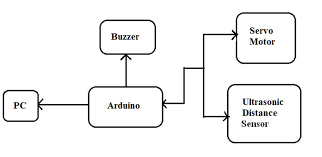
\includegraphics[scale=0.7]{block_diagram.png}
        \caption{\label{fig:pic}Block diagram for radar model}
    \end{figure}
    \linebreak
    \par You may ask how the processing application works here. It's very simple, the 
    Ultrasonic sensor collects the object information with the help of Arduino and passes 
    it to processing application, there is a simple Graphics application implemented which 
    mimic a radar screen.
    \subsection{Target Research}
        The short term goal of this topic is with the desire to learn and supplement the 
        knowledge that in the course of research. With the long term goal, i want to perform 
        the topic in the best way i can. As well as improve the errors of myselft. And also, 
        i want to additional the knowledge i haven't learned at my school.
    \subsection{Object and position research}
    \vspace{3mm}
        \begin{itemize}
            \item \textbf{Object Research:} The object that i study is the sensor system 
        installed on the air traffic control station or installed on robots that detect 
        objects and avoid them.
            \item \textbf{Position Research:} My reserach is based on the application of radar 
        to detect missing vehicles or to apply air traffic control as call as "Primary Surveillance Radar".
        \end{itemize} 
    \subsection{Method of research}
        \begin{itemize}
            \item \textbf{Observation Method:} By observing directly at air traffic control 
        and also via movies or aviation videos on internet.
            \item \textbf{Method of analysis:} Looking for some similar projects that have 
        been made available online, from the detailed data of those projects, i draw some 
        methods and experience for my project. Avoid mistakes in my project.
        \end{itemize}
    \subsection{Structure Project}
        My article is divided into three main sessions, summarized as follow: 
        \begin{itemize}
            \item In the first chapter, i will focus on brief introduce my project, presenting 
        some of the research content on the topic of the method of conducting research that 
        gives practical results during the project research process.
            \item The second chapter, is an introduction about some of basic project implementation 
        theories, to present related project i'm working on it.
            \item Chapter three is the chapter where i introduce the main content of my project, 
        presenting a basic article of project and how it works, accompany it with some examples.
            \item The next chapter is the construction and circuit design on Kicad Altium software 
        and the implementation of hardware construction.
            \item And the final chapter is the final section where i draw some conclusion during 
        project implementation, as well as point out my own strengths weaknesses in the course of my project.
        \end{itemize}
    \newpage
    \section{BASIC THEORY}
    \subsection{Some research related to the project}
        Some research ideas related to my project:
        \begin{itemize}
            \item The function contained in some robots, helps robots scan the terrain 
        and detect objects to avoid.
            \item Radar in the Air traffic control tower named "Primary Surveillance Radar"
        \end{itemize}
    \subsection{Theory concepts related to research issues}
        \begin{itemize}
            \item \textbf{PSR(Primary Surveillance Radar)}: A Surveillance radar system which
        uses reflected radio signals.
            \item \textbf{US(Ultrasonic Sensor)}: As the name indicates, ultrasonic sensors 
        measure distance by using ultrasonic waves.
            \item \textbf{PWM(Pulse-Width Modulation)}: is a method of reducing the average 
        power delivered by an electrical signal, by effectively chopping it up into discrete parts.
            \item \textbf{RAM(Random-Access Memory)}: is a form of computer memory that can be 
        read and changed in any order, typically used to store working data and machine code.
            \item \textbf{CPU(Central Processing Unit)}: also called a central processor or main 
        processor, is the electronic circuitry within a computer that executes instruction that 
        make up a computer program.
        \end{itemize}
    \subsection{Components Required}
        \begin{enumerate}
            \item For power:
            \setlength{\parindent}{4em}
            Micro USB-B
            \item For radar model:
            \begin{enumerate}
                \item Arduino UNO
                \item Servo motor
                \item Ultrasonic Sensor HRF-04
                \item Buzzer
                \item LCD 16x02
                \item LED (green, red)
                \item Test board
            \end{enumerate}
        \end{enumerate}
    \newpage
    \subsection{Component Description}
        \vspace{3mm}
        \subsubsection{Arduino Uno}
            \vspace{3mm}
            \begin{enumerate}
                \item \textbf{Introduction about Arduino UNO}
                \linebreak
                \par Arduino UNO is a microcontroller board developed by Arduino.cc which is open-source 
                electronics platform mainly based on AVR microcontroller ATMega328. \\
                \vspace{3mm}
                \par First Arduino projcet was started in Interaction Design Institute 
                Ivrea in 2003 by David Cuartielles and Massimo Banzi with the intention of 
                providing a cheap and flexible way to students and professional for controlling 
                a number of devices in the real world. \\
                \vspace{3mm}
                \par The current version of Arduino UNO comes with USB interface, 6 analog 
                input pins, 14 I/O(input/output) digital ports that are used to connect with 
                external electronic circuit. Out of 14 I/O ports, 6 pins can be used for PWM output.\\
                \vspace{3mm}
                \par It allows the designers to control and sense the external electronic devices in 
                the real world. \\
                \vspace{3mm}
                \par Apart from USB, battery or AC to DC adopter can also be used to power the board. \\
                \vspace{3mm}
                \par There are many versions of Uno board available. However, Arduino Uno V3 and Arduino 
                Uno are the most official versions that come with ATMega328 8-bit AVR Atmel microcontroller 
                where RAM memory is 32KB.
                \begin{figure}[ht]
                    \centering
                    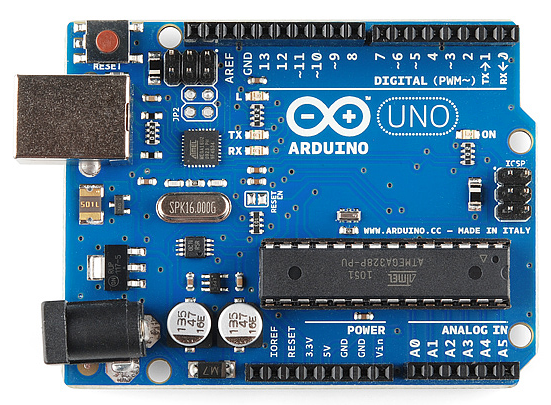
\includegraphics[width=0.5\linewidth]{Uno.png}
                    \caption{\label{fig:pic}Arduino Uno board}
                \end{figure}
                \item \textbf{Features}
                    \linebreak
                \begin{itemize}
                    \item Comes with USB interface.
                    \item USB port is added on the board to develop serial communication with the computer
                    \item ATMega328 microcontroller is placed on the board that comes with a number of 
                features like timers, counters, interrupts, PWM, CPU, I/O pins and based on a 16MHz clock 
                that helps in producing more frequency and number of instruction per cycle.
                    \item It's an open-source platform where anyone can modify and optimize the 
                board based on the number of instructions and task they want to achieve.
                    \item Come with a built-in regulation feature which keeps the voltage under control 
                when the device is connected to the external device.
                    \item There are 14 pins I/O digital and 6 analog pins in the board that allows the 
                external connection with any circuit with the board. These pins provide the flexibility 
                and ease of use to the external devices that can be connected through these pins.
                    \item 6 analog pins are marked as A0 to A5 and come with a resolution of 10bits. 
                These pins measure from 0V to 5V, however, they can be configured to the high range 
                using analogReference() function and AREF pin.
                    \item 13KB of flash memory is used to store the number of instructions in the form 
                of code.
                    \item Only 5V is required to turn the board on, which can be achieved directly using 
                USB port or external adopter, however, it can support external power source up to 12V 
                which can be regulated and limit to 5V or 3.3V based on the requirement of the project. 
                \end{itemize}
                \item \textbf{Pinout}
                    \linebreak
                    \vspace{3mm}
                    \par Arduino Uno is based on AVR microcontroller call ATMega328. This controller 
                comes with 2KB RAM, 32KB of flash memory, 1KB of EEPROM. Arduino board comes with 
                14 digital pins and 6 analog pins.
                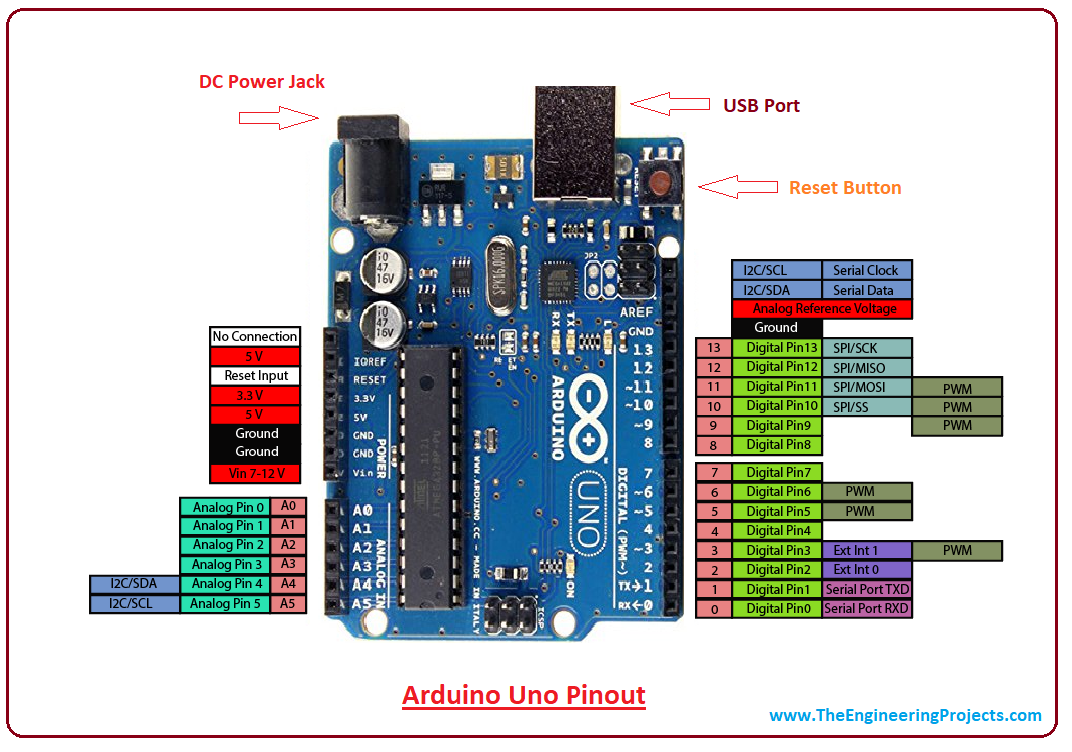
\includegraphics[width=\linewidth]{pinout.png}
                \item \textbf{Pin Description}
                    \linebreak
                    \vspace{3mm}
                    \par \textbf{LED:} comes with build-in LED which is connected through pin 13.
                Providing HIGH value to the pin will turn it ON and LOW will turn it OFF. \\
                    \vspace{2mm}
                    \par \textbf{Vin:} input voltage provided to the Arduino Uno board. It's
                different than 5V supplied through the USB port. This pin is used to supply voltage. 
                If a voltage is provided through power jack, it can be accessed through this pin. \\
                    \vspace{2mm} 
                    \par \textbf{5V:} comes with the ability to provide voltage regulation. 5V pin is 
                used to provide output regulated voltage. The board is powered up using the 3 ways: 
                USB, Vin pin of the board or DC power jack.
            \end{enumerate}
\end{document}